\section{Aktienoptionen}

\subsection{Finanzmathematische Grundlagen}

Aktienoptionen sind Finanzderivate, die dem Inhaber das Recht, aber nicht die Pflicht geben, 
eine Aktie zu einem vorher festgelegten Preis (dem Ausübungspreis) zu kaufen (Call-Option) 
oder zu verkaufen (Put-Option). Europäische Optionen können nur am Fälligkeitstag ausgeübt 
werden, während amerikanische Optionen während der gesamten Laufzeit bis zum Verfallsdatum 
ausgeübt werden können. Ein zentrales Konzept ist die Put-Call-Parität, die eine Beziehung 
zwischen dem Preis einer europäischen Call- und Put-Option mit identischem Basiswert, 
Ausübungspreis und Laufzeit herstellt. Den fairen Preis einer Option zu bestimmen ist eine Herausforderung,
die man mit Hilfe der geometrischen Brownschen Bewegung lösen kann. Im Folgenden wird dazu das Black-Scholes-Modell 
vorgestellt.

\begin{bsp}
\textit{Beispiel Call-Option.} 
Ein Investor erwirbt eine europäische Call-Option auf die Aktie der Firma X mit einem
 Ausübungspreis von 50\,€. Am Fälligkeitstag steht der Aktienkurs bei 60\,€. 
 Der Investor übt die Option aus, kauft die Aktie für 50\,€ und kann 
 sie sofort für 60\,€ verkaufen. Sein Gewinn (ohne Berücksichtigung der Optionsprämie) 
 beträgt 10\,€ pro Aktie.\\
\textit{Motivation.} Der Investor spekuliert darauf, dass der Kurs der Aktie steigt 
und über den Ausübungspreis hinausgeht.

\textit{Beispiel Put-Option.}
Ein Landwirt sichert sich gegen fallende Weizenpreise ab und kauft eine europäische 
Put-Option mit einem Ausübungspreis von 200\,€/Tonne. Am Fälligkeitstag liegt der 
Marktpreis bei 170\,€/Tonne. Der Landwirt übt die Option aus und verkauft seinen 
Weizen zum höheren Preis von 200\,€/Tonne, obwohl der Marktpreis niedriger ist. 
Sein Vorteil beträgt 30\,€ pro Tonne (abzüglich der Optionsprämie).
\end{bsp}
% 
\subsection{Bewertung von Aktienoptionen im Binomialmodell}

Das Binomialmodell wird erweitert. Zusätzlich zur Aktie und deren Kurs gibt es nun die Bank, die einen risikofreien Zinssatz $r$ anbietet.

\begin{defi}[Arbitrage-Prinzip]
Es wird angenommen, dass man keine risikolosen Gewinne erzielen kann, ohne Kapital zu investieren.
\end{defi}

\begin{defi}[Europäische Optionen]
    Europäische Optionen sind Finanzderivate, die dem Inhaber das Recht geben, 
    einen Basiswert zu einem festgelegten Preis (dem Ausübungspreis) nur am 
    Fälligkeitstag zu kaufen (Call-Option) oder zu verkaufen (Put-Option).
    Der Wert einer europäischen Call-Option am Endzeitpunkt $T$ ist durch die Auszahlungsfunktion
    $$f(S_T) = \max(S_T - K, 0) = (S_T - K)^+$$
    gegeben, wobei $K$ der Ausübungspreis ist.
    Für eine Put-Option ist die Auszahlungsfunktion
    $$\tilde f(S_T) = \max(K - S_T, 0) = (K - S_T)^+.$$
Das entspricht der \textit{Call-Put-Parität}
    $f(S_T) - \tilde f(S_T) = S_T - K$.
\end{defi}


\begin{lemma}[Risikoneutrale Wahrscheinlichkeit für einen Schritt]
Da in diesem Fall die Aussicht auf Zinsen berücksichtigt werden muss,
werden mögliche Aktiengewinne mit dem Faktor $e^{r \Delta t}$ verkleinert (diskontiert).
Der diskontierte Aktienkurs zum Zeitpunkt $n$ ist $e^{-r n \Delta t} S_n$.
Im Folgenden wird berechnet, für welche Wahrscheinlichkeit der neue diskontierte Prozess
ein Martingal ist. Das Martingal-Kriterium lautet: $E(X_{n+1} \mid X_n = l) = l$, wobei $X_n = e^{-r n \Delta t} S_n$.
Einsetzen von $X_{n+1} = e^{-r (n+1) \Delta t} S_{n+1}$ und $X_n = e^{-r n \Delta t} S_n$ ergibt
$$
E(e^{-r (n+1) \Delta t} S_{n+1} \mid S_n = v) = e^{-r n \Delta t} v
$$
Aus der Linearität des Erwartungswerts folgt
$$
E(e^{-r \Delta t} S_{n+1} \mid S_n=v) = v.
$$
Setzt man die möglichen Werte für $S_{n+1}$ ein ($S_{n+1} = u S_n$ mit Wahrscheinlichkeit $q$, $S_{n+1} = d S_n$ mit Wahrscheinlichkeit $1-q$) folgt
$$
e^{-r \Delta t} \left( q u S_n + (1-q) d S_n \right) = v.
$$
Teilt man durch $S_n = v$ ($v > 0$) ergibt sich
$$
e^{-r \Delta t} \left( q u + (1-q) d \right) = 1.
$$
Das ist äquivalent zu
$$
q = \frac{e^{r \Delta t} - d}{u - d}.
$$
Zum Vergleich: im klassischen Binomialmodell ist 
$$p = \frac{1 - d}{u - d}$$
die "risikoneutrale Wahrscheinlichkeit". Anders als zuvor
wurde aber lediglich eine schwächere Aussage gezeigt (nur ein Schritt). 
Das wird am Folgenden jedoch nachgezogen.

\end{lemma}

\begin{defi}[Risikoneutrales Maß]
Die soeben berechnete Wahrscheinlichkeit $q$ wird als risikoneutrales Maß bezeichnet.
Es handelt sich um ein diskretes Wahrscheinlichkeitsmaß $Q$ auf dem Wahrscheinlichkeitsraum des Binomialmodells,
wobei $Q(\text{up})=q$ und $Q(\text{down})=1-q$ gilt. In der Finanzmathematik kann das
riskoneutrale Maß oft nicht explizit angegeben werden, sondern über Existenz- und Eindeutigkeitstheoreme
charakterisiert werden, zum Beispiel mit dem Satz von Radon-Nikodym (XXX). Im Folgenden gilt:
$Q$ ist das Maß, für das das erweiterte Binomialmodell ein arbitragefreies Modell ist, das 
heißt der zugehörige stochastische Prozess ein Martingal ist. Die Existenz und Eindeutigkeit
wird hier nicht bewiesen.
\end{defi}

\begin{lemma}[Diskontierter Aktienkurs ist unter $Q$ ein Martingal]
Setze $X_n := e^{-r n \Delta t}\, S_n$. Unter dem risikoneutralen Maß $Q$ mit 
$q=\frac{e^{r\Delta t}-d}{u-d}$ ist $(X_n)_{n\in\mathbb N_0}$ ein Martingal.

\textit{Beweis.} Schreibe $S_{n+1}=S_n\,\xi_{n+1}$ mit 
$\mathbb P_Q(\xi_{n+1}=u)=q$ und $\mathbb P_Q(\xi_{n+1}=d)=1-q$. Für einen Schritt gilt
$$
\begin{aligned}
E_Q(X_{n+1}\mid S_n=v)
&= E_Q\!\big(e^{-r(n+1)\Delta t} S_{n+1}\mid S_n=v\big) \\
&= e^{-r(n+1)\Delta t}\, v \, E_Q(\xi_{n+1})
= e^{-rn\Delta t}\, v \cdot \big(e^{-r\Delta t}(q u + (1-q)d)\big).
\end{aligned}
$$
Mit der Wahl von $q$ ist $e^{-r\Delta t}(q u + (1-q)d)=1$, also 
$$E_Q(X_{n+1}\mid S_n=v)=e^{-rn\Delta t} v = X_n.$$
Für $s<t$ beliebig und wegen Unabhängigkeit der Schritte:
$$
X_t
= e^{-rt\Delta t} S_t
= e^{-rt\Delta t} S_s \prod_{i=s+1}^{t} \xi_i,
$$
also
$$
\begin{aligned}
E_Q(X_t\mid S_s=v)
&= e^{-rt\Delta t}\, v \prod_{i=s+1}^{t} E_Q(\xi_i)
= e^{-rt\Delta t}\, v \big(q u + (1-q)d\big)^{t-s} \\
&= e^{-rt\Delta t}\, v \big(e^{r\Delta t}\big)^{t-s}
= e^{-rs\Delta t}\, v
= X_s.
\end{aligned}
$$
Damit ist $(X_n)$ ein Martingal. \qed
\end{lemma}

\begin{satz}[Bewertung von europäischen Optionen im Binomialmodell]
Der Preis einer Option durch rekursive Rückwärtsinduktion bestimmt. 
Der Wert einer europäischen Option am Endzeitpunkt $T$ ist durch die Auszahlungsfunktion $f(S_T)$ gegeben, z.\,B.\ für eine Call-Option $f(S_T) = \max(S_T - K, 0)$.
Die Bewertung erfolgt rekursiv rückwärts:
$$
C_n = e^{-r \Delta t} \left( q C_{n+1}^\text{up} + (1-q) C_{n+1}^\text{down} \right),
$$
wobei $C_{n+1}^\text{up}$ und $C_{n+1}^\text{down}$ die Optionswerte im nächsten Schritt nach Auf- bzw. Abbewegung sind.
Damit lässt sich der Optionspreis am Anfangszeitpunkt $C_0$ bestimmen. Die Formel leitet
sich aus dem Ewartungswert unter dem risikoneutralen Maß $Q$ ab, dessen Verhalten im ein-stufigen Fall ja explizit bekannt ist.
Der faire Preis der Option ist der Erwartungswert der diskontierten Auszahlung (unter dem risikoneutralen Maß).
\end{satz}

\begin{bsp}
Seien $S_0 = 100\,€$, $u=1.2$, $d=0.8$, $r=0.05$, $\Delta t=1$ Jahr, $K=100\,€$ und $T=2$ Jahre.
Die risikoneutrale Wahrscheinlichkeit ist $q = \frac{e^{0.05}-0.8}{1.2-0.8} \approx 0.628$.
Die möglichen Aktienkurse zum Zeitpunkt $T$ sind:
\begin{tikzpicture}[x=3.2cm,y=1.4cm,>=stealth]
    % styles
    \tikzset{price/.style={circle,draw,minimum size=6mm,inner sep=0pt,font=\small}}
    % nodes
    \node[price] (S0)  at (0,0)   {100};
    \node[price] (Su)  at (1,1)   {120};
    \node[price] (Sd)  at (1,-1)  {80};
    \node[price] (Suu) at (2,2)   {144};
    \node[price] (Sud) at (2,0)   {96};
    \node[price] (Sdd) at (2,-2)  {64};

    % edges with risk-neutral probabilities
    \draw[->] (S0) -- node[sloped,above] {$q$} (Su);
    \draw[->] (S0) -- node[sloped,below] {$1-q$} (Sd);

    \draw[->] (Su) -- node[sloped,above] {$q$} (Suu);
    \draw[->] (Su) -- node[sloped,below] {$1-q$} (Sud);

    \draw[->] (Sd) -- node[sloped,above] {$q$} (Sud);
    \draw[->] (Sd) -- node[sloped,below] {$1-q$} (Sdd);

    % time axis labels
    \node[font=\scriptsize] at (0,-2.4) {Zeit 0};
    \node[font=\scriptsize] at (1,-2.4) {Zeit 1};
    \node[font=\scriptsize] at (2,-2.4) {Zeit 2 = T};

    % parameter box
    \node[anchor=west, align=left, font=\scriptsize] at (2.6,2.0) {Parameter:\\
        $u=1.2,\; d=0.8$\\
        $r=0.05,\; \Delta t=1$\\
        $q \approx 0.628$
    };
\end{tikzpicture} \\ Die Auszahlungen der Call-Option zum Zeitpunkt $T$ sind:
$$
\begin{aligned}
C_{T,\text{up}} &= \max(144 - 100, 0) = 44\,€, \\
C_{T,\text{mid}} &= \max(96 - 100, 0) = 0\,€, \\
C_{T,\text{down}} &= \max(64 - 100, 0) = 0\,€.
\end{aligned}
$$
Rückwärtsinduktion:
$$
\begin{aligned}
C_{1,\text{up}} &= e^{-0.05} \left( q \cdot 44 + (1-q) \cdot 0 \right) \approx 26.28\,€, \\
C_{1,\text{down}} &= e^{-0.05} \left( q \cdot 0 + (1-q) \cdot 0 \right) = 0\,€, \\
C_0 &= e^{-0.05} \left( q \cdot 23.99 + (1-q) \cdot 0 \right) \approx 15.7\,€.
\end{aligned}
$$
Der faire Preis der Call-Option ist also etwa 15.7\,€.
\end{bsp}

\subsection{Das Black-Scholes-Modell als Grenzfall des Binomialmodells}
Ziel ist es zu zeigen, dass die Optionspreise im Binomialmodell
beim Verfeinern der Zeitdiskretisierung gegen die geometrische Brownsche Bewegung konvergieren.
Dieses Modell wird auch als Black-Scholes-Modell bezeichnet. Die Herleitung unterscheidet sich
von der Herleitung in Kapitel 2. Hier wird der Grenzübergang im risikoneutralen Maß durchgeführt.

\paragraph{Vereinfachung der risikoneutralen Wahrscheinlichkeit im Grenzübergang}
Wähle für Zeitschritt $\Delta t$ die Sprunggrößen
$
u = e^{\sigma \sqrt{\Delta t}},\quad d = e^{-\sigma \sqrt{\Delta t}}
$
und den risikoneutralen Schritt $q(\Delta t)$ aus dem Martingal-Kriterium
$$
q(\Delta t) = \frac{e^{r \Delta t} - d}{u - d}
= \frac{e^{r \Delta t} - e^{-\sigma \sqrt{\Delta t}}}{e^{\sigma \sqrt{\Delta t}} - e^{-\sigma \sqrt{\Delta t}}}.
$$
\\ Durch eine Taylor-Entwicklung um $0$ werden die Funktionen wieder vereinfacht. Analog zum Beweis aus Kapitel 2
sollen höhere Potenzen von $\Delta t$ im Grenzwert verschwinden. Da es sich um einen Quotienten handelt,
kann man die Abschätzung aber nicht direkt anwenden. Stattdessen werden Zähler und Nenner separat entwickelt:
$$
e^{r\Delta t} = 1 + r\Delta t + o(\Delta t),\quad
e^{\pm \sigma\sqrt{\Delta t}} = 1 \pm \sigma \sqrt{\Delta t} + \tfrac12 \sigma^2 \Delta t + o(\Delta t).
$$
Damit
$$
\begin{aligned}
\text{Zähler} &= e^{r \Delta t} - e^{-\sigma \sqrt{\Delta t}}
= \big(1 + r\Delta t + o(\Delta t)\big) - \big(1 - \sigma \sqrt{\Delta t} + \tfrac12 \sigma^2 \Delta t + o(\Delta t)\big) \\
&= \sigma \sqrt{\Delta t} + \big(r - \tfrac12 \sigma^2\big)\Delta t + o(\Delta t), \\
\text{Nenner} &= e^{\sigma \sqrt{\Delta t}} - e^{-\sigma \sqrt{\Delta t}}
= \big(1 + \sigma \sqrt{\Delta t} + \tfrac12 \sigma^2 \Delta t + o(\Delta t)\big) \\
&\qquad\qquad\qquad - \big(1 - \sigma \sqrt{\Delta t} + \tfrac12 \sigma^2 \Delta t + o(\Delta t)\big)
= 2\sigma \sqrt{\Delta t} + o(\sqrt{\Delta t}).
\end{aligned}
$$
Insgesamt folgt damit:
$$
q(\Delta t) = \frac{\sigma \sqrt{\Delta t} + \big(r - \tfrac12 \sigma^2\big)\Delta t + o(\Delta t)}{2\sigma \sqrt{\Delta t} + o(\sqrt{\Delta t})}
= \tfrac12 + \frac{r - \tfrac12 \sigma^2}{2\sigma}\,\sqrt{\Delta t} + o(\sqrt{\Delta t}).
$$

\paragraph{Erneute Herleitung der geometrischen Brownschen Bewegung}
An dieser Stelle ist wichtig, dass die Anzahl der Schritte $N_u$ in denen die Aktie steigt, binomialverteilt ist.
Und zwar zur Anzahl der Schritte $n=T/\Delta t$ mit festen Wahrscheinlichkeit $q(\Delta t)$.
Dann gilt
$$
S_T^{(n)} = S_0\, u^{N_u}\, d^{n-N_u}
\approx S_0 \exp\!\big(\sigma \sqrt{\Delta t}\,(2N_u - n)\big).
$$
Und somit
$$
\log S_T^{(n)}
= \log S_0 + \sigma \sqrt{\Delta t}\,(2N_u - n).
$$
Es wird eine 0 addiert:
$$
2N_u - n
= 2\big(N_u - n q(\Delta t)\big) + n\big(2q(\Delta t)-1\big).
$$
Zwischenfazit:
$$
\log S_T^{(n)}
= \log S_0 + \sigma \sqrt{\Delta t}\, n\big(2q(\Delta t)-1\big)
+ \sigma \sqrt{\Delta t}\, 2\big(N_u - n q(\Delta t)\big).
$$
Zuerst wird der stochastische Term (rechts) untersucht: Da die Binomialverteilung eine Summe von unabhängigen Bernoulli-Verteilungen ist, kann der zentrale Grenzwertsatz angewendet werden:
$$
\lim_{n\to\infty} N_u = \lim_{n \to \infty} \sum_{k=0}^{n}\text{Ber}(q(\Delta t)) \sim \mathcal N\big(n q(\Delta t), n q(\Delta t)(1-q(\Delta t))\big).
$$
Das ist äquivalent zu
$$
\frac{N_u - n q(\Delta t)}{\sqrt{n\,q(\Delta t)(1-q(\Delta t))}} \longrightarrow Z\sim \mathcal N(0,1),
$$
also
$$
2\big(N_u - n q(\Delta t)\big) = 2\sqrt{n\,q(\Delta t)(1-q(\Delta t))}\,Z_n,
$$
wobei $Z_n\longrightarrow Z$.
Schließlich folgt aus $q(\Delta t)\to \tfrac12$ für $\Delta t\to 0$:
$$
\begin{aligned}
\sigma \sqrt{\Delta t}\cdot 2\sqrt{n\,q(\Delta t)(1-q(\Delta t))}\,Z_n
&= 2\sigma \sqrt{n\Delta t}\,\sqrt{q(\Delta t)(1-q(\Delta t))}\,Z_n \\
&= 2\sigma \sqrt{T}\,\sqrt{\tfrac14 + o(1)}\,Z_n
= \sigma \sqrt{T}\,Z_n + o(1).
\end{aligned}
$$
Nun wird der deterministische Term (mittig) untersucht:
\\ Multipliziere mit $\sigma \sqrt{\Delta t}$ und benutze $n\Delta t=T$ sowie $q(\Delta t)=\tfrac12 + \alpha \sqrt{\Delta t} + o(\sqrt{\Delta t})$ mit
$\alpha=\frac{r-\frac12\sigma^2}{2\sigma}$:
$$
\begin{aligned}
\sigma \sqrt{\Delta t}\, n\big(2q(\Delta t)-1\big)
&= \sigma \sqrt{\Delta t}\, n\big(2\alpha \sqrt{\Delta t} + o(\sqrt{\Delta t})\big)
= \sigma\, n \big(2\alpha \Delta t + o(\Delta t)\big) \\
&= \sigma \cdot 2\alpha \cdot (n\Delta t) + o(1)
= \big(r - \tfrac12 \sigma^2\big)T + o(1).
\end{aligned}
$$
Zwischenfazit:
$$
\log S_T^{(n)}
= \log S_0 + \big(r - \tfrac12 \sigma^2\big)T + \sigma \sqrt{T}\,Z_n + o(1).
$$
Im Grenzwert $n\to\infty$ (bzw.\ $\Delta t \to 0$) folgt damit
$$
\log S_T \sim \mathcal N\!\Big(\log S_0 + \big(r - \tfrac12 \sigma^2\big)T,\;\sigma^2 T\Big),
$$
d.\,h.\ unter $Q$ konvergiert der diskrete Prozess gegen die geometrische Brownsche Bewegung.
\qed

\begin{satz}[Satz von Pratt, Elstrod S. 280, vereinfacht]
Dieser technische Satz erlaubt es, den Grenzübergang und den Erwartungswert zu vertauschen, und
kommt im Folgenden bei der Herleitung der Black-Scholes-Formel zum Einsatz.
Sei $(X_n) \longrightarrow X$ eine Folge von Zufallsvariablen, die fast-überall konvergiert,
und $(Y_n) \longrightarrow Y$, $(Z_n) \longrightarrow Z$ ebenfalls.
Gilt (1) $Y_n \le X_n \le Z_n$ und (2) $E(Y_n) \longrightarrow E(Y)$, $E(Z_n) \longrightarrow E(Z)$,
dann folgt $E(X_n) \longrightarrow E(X)$. Wird hier nicht bewiesen. \qed
\end{satz}

\begin{satz}[Black–Scholes-Formel für europäische Call-Optionen]
Sei $C_0^{(n)}$ der Preis der europäischen Call-Option mit Laufzeit $T$ und Strike $K$
im $n$-stufigen Binomialmodell unter Diskontierung mit $r$. Dann gilt
$$
\lim_{n\to\infty} C_0^{(n)}
= C_0^{\mathrm{BS}}
= S_0\,\Phi(d_1) - K e^{-rT}\,\Phi(d_2),
$$
wobei
$$
d_1 = \frac{\ln(S_0/K) + \big(r + \tfrac12 \sigma^2\big)T}{\sigma \sqrt{T}},
\qquad
d_2 = d_1 - \sigma \sqrt{T},
$$
und $\Phi$ die Verteilungsfunktion der Standardnormalverteilung ist.
\\ \textit{Beweis}. Risikoneutrale Bewertung im Binomialmodell liefert
$$
C_0^{(n)} = e^{-rT}\,E\!\left[(S_T^{(n)} - K)^+\right].
$$
Die obige Verteilungskonvergenz impliziert
$$
S_T^{(n)} \longrightarrow S_T = S_0 \exp\!\big((r-\tfrac12\sigma^2)T + \sigma \sqrt{T}\,Z\big).
$$
Nun wird der Satz von Pratt angewendet, um den Grenzübergang und den Erwartungswert zu vertauschen. Eine untere Schranke ist $Y_n=0$ und eine obere Schranke ist $Z_n = (S_T^{(n)})^+ = S_T^{(n)}$. 
$$
\lim_{n\to\infty} C_0^{(n)} = e^{-rT}\,E\!\left[ h(\lim_{n\to\infty} S_T^{(n)}) \right] = e^{-rT}\,E_Q\!\left[(S_T - K)^+\right].
$$
Nun wird die rechte Seite explizit berechnet: Seien
$$
m := \big(r-\tfrac12\sigma^2\big)T,\qquad v:=\sigma \sqrt{T},\qquad Z\sim \mathcal N(0,1),
$$
also $S_T = S_0 e^{m + v Z}$. Dann gilt
$$
E\big[(S_T - K)^+\big]
= E\big[S_T\,\mathbf 1_{\{S_T\ge K\}}\big] - K\,P(S_T\ge K).
$$
Aus Kapitel 2 ist bekannt, das $S_T$ lognormalverteilt ist. Die Schranke $S_T\ge K$ ist daher äquivalent zu $m + vZ \ge \ln(K/S_0)$, also
$$
Z \ge a := \frac{\ln(K/S_0) - m}{v}.
$$
Damit ergibt sich für den zweiten Term
$$
P(S_T\ge K) = P(Z\ge a) = \Phi(-a).
$$
Für den ersten Term wird die Dichte $\varphi$ von $Z$ genutzt:
$$
\begin{aligned}
E\big[S_T\,\mathbf 1_{\{Z\ge a\}}\big]
&= S_0 e^{m}\int_a^\infty e^{v x}\,\varphi(x)\,dx
= S_0 e^{m}\int_a^\infty e^{v x}\,\frac{1}{\sqrt{2\pi}}e^{-x^2/2}\,dx \\
&= S_0 e^{m}\int_a^\infty \frac{1}{\sqrt{2\pi}}
\exp\!\Big(-\tfrac12(x^2 - 2 v x)\Big)\,dx \\
&= S_0 e^{m}\int_a^\infty \frac{1}{\sqrt{2\pi}}
\exp\!\Big(-\tfrac12(x - v)^2 + \tfrac12 v^2\Big)\,dx \\
&= S_0 e^{m + \frac12 v^2}\int_a^\infty \varphi(x - v)\,dx.
\end{aligned}
$$
Mit der Substitution $y=x-v$ folgt
$$
\int_a^\infty \varphi(x - v)\,dx = \int_{a-v}^\infty \varphi(y)\,dy = \Phi(v-a).
$$
Zwischenfazit:
$$
E\big[S_T\,\mathbf 1_{\{S_T\ge K\}}\big]
= S_0 e^{m + \frac12 v^2}\,\Phi(v-a).
$$
Setze $m+\tfrac12 v^2 = rT$ und beachte
$$
v-a = \frac{\ln(S_0/K) + (r+\tfrac12\sigma^2)T}{\sigma \sqrt{T}} = d_1,
\qquad
-a = \frac{\ln(S_0/K) + (r-\tfrac12\sigma^2)T}{\sigma \sqrt{T}} = d_2.
$$
Damit gilt
$$
E\big[(S_T - K)^+\big]
= S_0 e^{rT}\,\Phi(d_1) - K\,\Phi(d_2),
$$
und folglich
$$
C_0^{\mathrm{BS}} = e^{-rT}\,E\big[(S_T - K)^+\big]
= S_0\,\Phi(d_1) - K e^{-rT}\,\Phi(d_2).
$$
\qed
\end{satz}

\begin{bem}
Für den europäischen Put folgt analog
$$
P_0^{\mathrm{BS}} = K e^{-rT}\,\Phi(-d_2) - S_0\,\Phi(-d_1),
$$
oder per Put-Call-Parität.

\end{bem}
\begin{bem}

Der Drift $\mu$ der Aktie spielt im in der Formel keine Rolle.
Eine Option "wettet" ja nicht auf den tatsächlichen (erwarteten) Kursverlauf, sondern darauf,
dass der Kurs über oder unter dem Ausübungspreis liegt.

\end{bem}

\begin{bsp}[Call-Option auf den DAX]
Mit der zuvor geschätzten Volatilität ($\sigma$) des DAX kann
man nun den Preis einer Call-Option auf den DAX berechnen. Das folgende
R-Programm (Ausschnitt) berechnet den Preis einer Call-Option abhängig
vom Ausübungspreis $K$.

\begin{lstlisting}
d1 <- (log(S0/K) + (r + 0.5 * sigma^2) * T) / (sigma * sqrt(T))
d2 <- d1 - sigma * sqrt(T)
C <- S0 * pnorm(d1) - K * exp(-r*T) * pnorm(d2)
\end{lstlisting}
Ein Beispiel mit $r = 0.02, T = 1$ Jahr und dem DAX-Stand $S_0 = 24290$ wird in
der folgenden Grafik dargestellt. Der faire Preis der Option
fällt (erwartungsgemäß) mit dem Ausübungspreis $K$.


\begin{figure}[H]
    \centering
    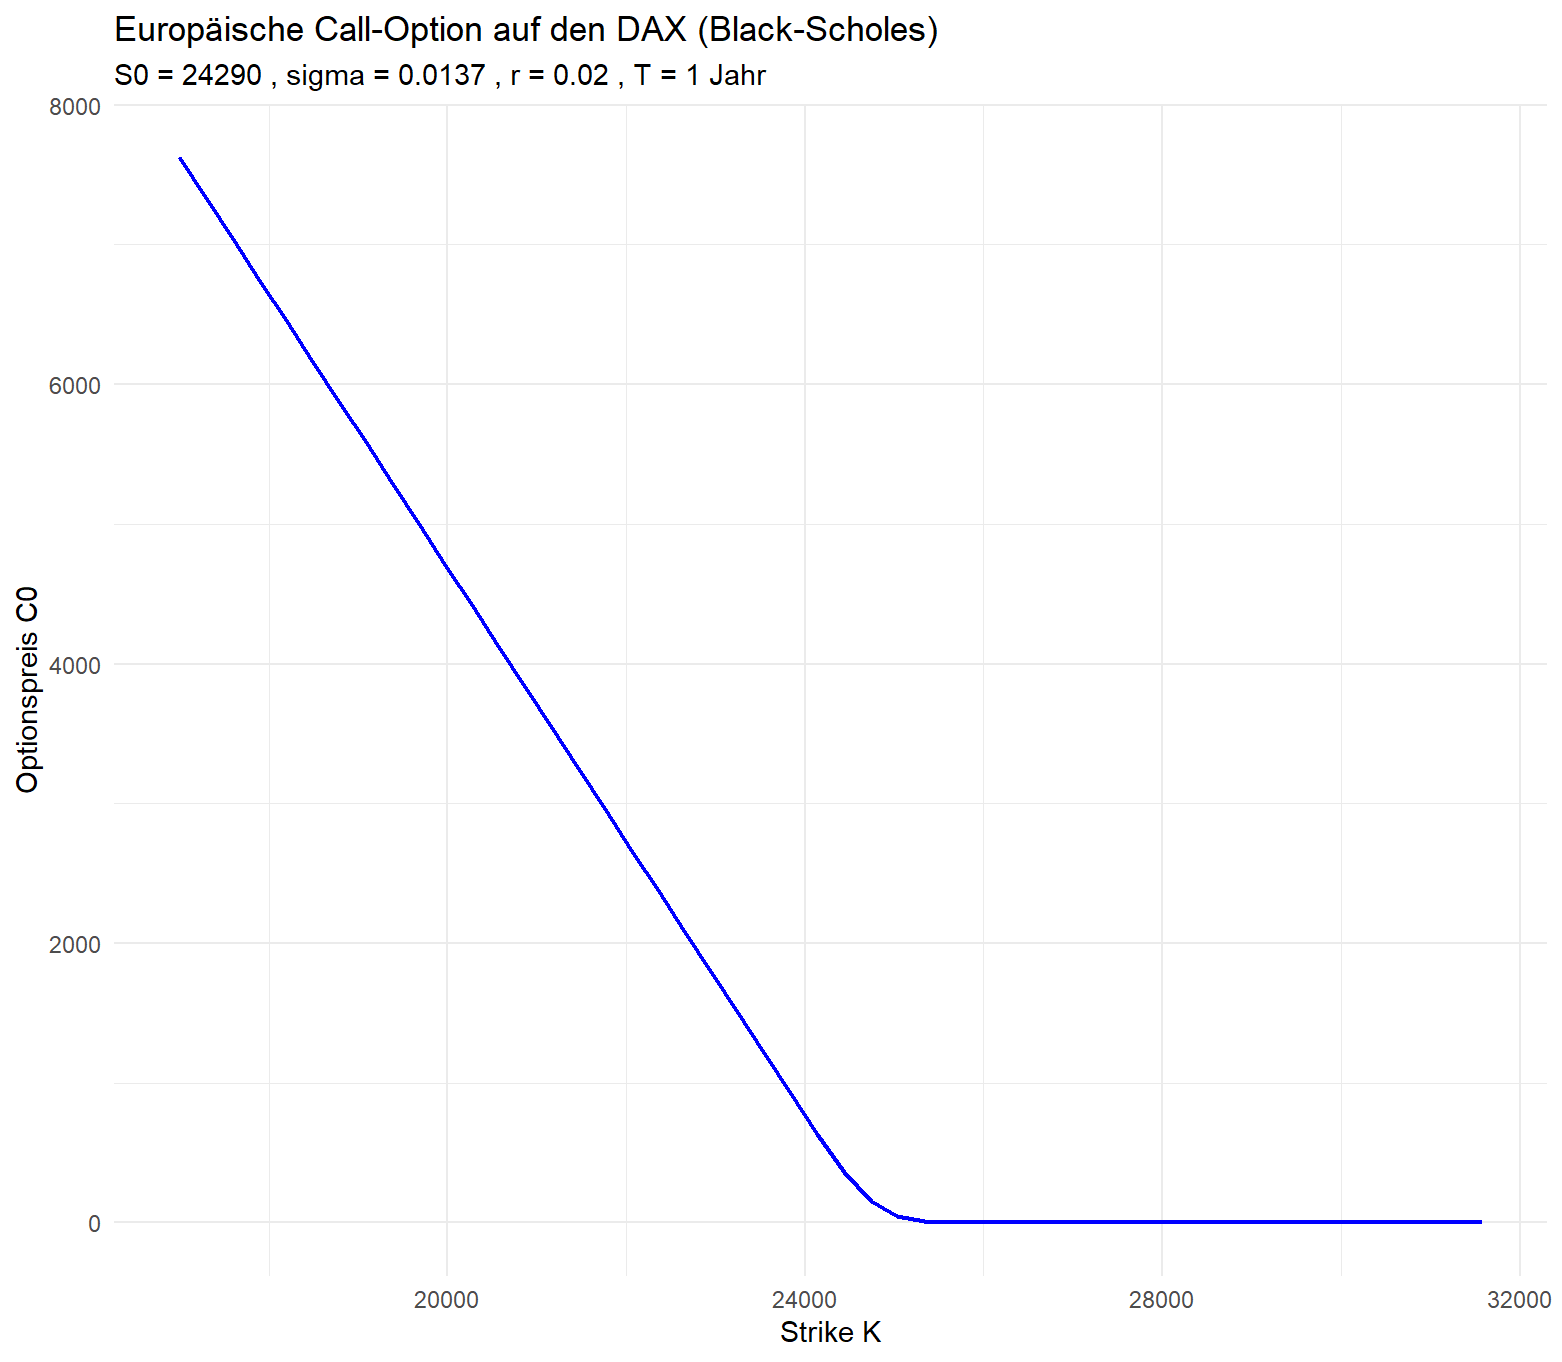
\includegraphics[width=0.9\textwidth]{images/call_dax_bs.png}
    \caption{Preis einer Call-Option auf den DAX in Abhängigkeit vom Ausübungspreis $K$}
    \label{fig:call_dax_bs}
\end{figure}

\end{bsp}

\subsection{Bewertung von Aktienoptionen mit Monte-Carlo-Verfahren}
Der letzte Beweis zeigt, dass explizite Formeln für Optionspreise nur mit hohem
Aufwand hergeleitet werden können. Man bedenke, dass es sich um eine 
vergleichsweise simple Option gehandelt hat. Für komplexere Derivate
gibt es meist keine geschlossenen Formeln. Stattdessen werden numerische Verfahren
verwendet, um den Erwartungswert der diskontierten Auszahlung zu approximieren.

\begin{defprop}[Monte-Carlo-Verfahren]
Monte-Carlo-Verfahren sind stochastische Simulationsmethoden, die zur numerischen
Lösung von Problemen verwendet werden, insbesondere zur Berechnung von Integralen
und Erwartungswerten. Sie basieren auf der Erzeugung von Zufallszahlen und
der statistischen Analyse der Ergebnisse. Man verwendet den \textit{Monte-Carlo-Schätzer}
$$
\hat{I}_n = \frac{1}{n} \sum_{i=1}^n f(X_i),
$$
wobei $X_1, X_2, \ldots, X_n$ unabhängige und identisch verteilte Zufallsvariablen
sind, die der Verteilung von $X$ folgen. Der Schätzer konvergiert fast sicher
gegen den wahren Erwartungswert $I = E[f(X)]$, wenn $n \to \infty$.
\textit{Beweis.} Nach dem Gesetz der großen Zahlen gilt
$$\hat{I}_n \longrightarrow E[f(X)] = I. \quad \text{fast sicher}$$
\qed
\end{defprop}

\begin{lemma}[Anwendung auf Optionspreise]
Um allgemeine Optionen zu bewerten, muss die Auszahlungsfunktion $f$
nicht bloß relle Zahlen auf relle Zahlen abbilden, sondern des gesamten Pfad
$S_t$, $t\in[0,T]$ auf reelle Zahlen Abbilden. Bei z. B. asiatischen Optionen ist
der Durchschnittskurs über die Laufzeit relevant.
Sei also im Folgenden 
$$f: C([0,T]) \to \mathbb R, \tilde S_T \mapsto f(\tilde S_T)$$
eine Auszahlungsfunktion. Der faire Option mit Auszahlung $f(S_T)$
unter dem risikoneutralen Maß $Q$ ist
$$
C_0 = e^{-rT} E_Q[f(S_T)].
$$
Der Monte-Carlo-Schätzer für $C_0$ ist somit
$$
\hat{C}_0^{(n)} = e^{-rT} \frac{1}{n} \sum_{i=1}^n f(S_T^{(i)}),
$$
wobei $S_T^{(i)}$, $i=1,\ldots,n$ unabhängige Realisierungen des Prozesses $S_T$ sind.

\end{lemma}

\begin{bsp}[Monte-Carlo-Simulation einer Call-Option auf den DAX]

Das folgende R-Programm simuliert den Preis einer Call-Option auf den DAX
mit dem Monte-Carlo-Verfahren. Dabei wird die geometrische Brownsche Bewegung
simuliert und der Erwartungswert der diskontierten Auszahlung approximiert.

\begin{lstlisting}
  Z <- rnorm(n)
  ST <- S0 * exp((r - 0.5*sigma^2)*T + sigma*sqrt(T)*Z)
  payoff <- pmax(ST - K, 0) # Bewertungsfunktion
  C <- exp(-r*T) * mean(payoff)
\end{lstlisting}
Nun wird der simulierte Preis mit dem Preis aus der Black-Scholes-Formel verglichen. 
Die folgende Grafik zeigt den Vergleich für verschiedene Ausübungspreise $K$.
Je höher die Anzahl der Simulationen $n$, desto genauer ist die Approximation.

\begin{figure}[H]
    \centering
    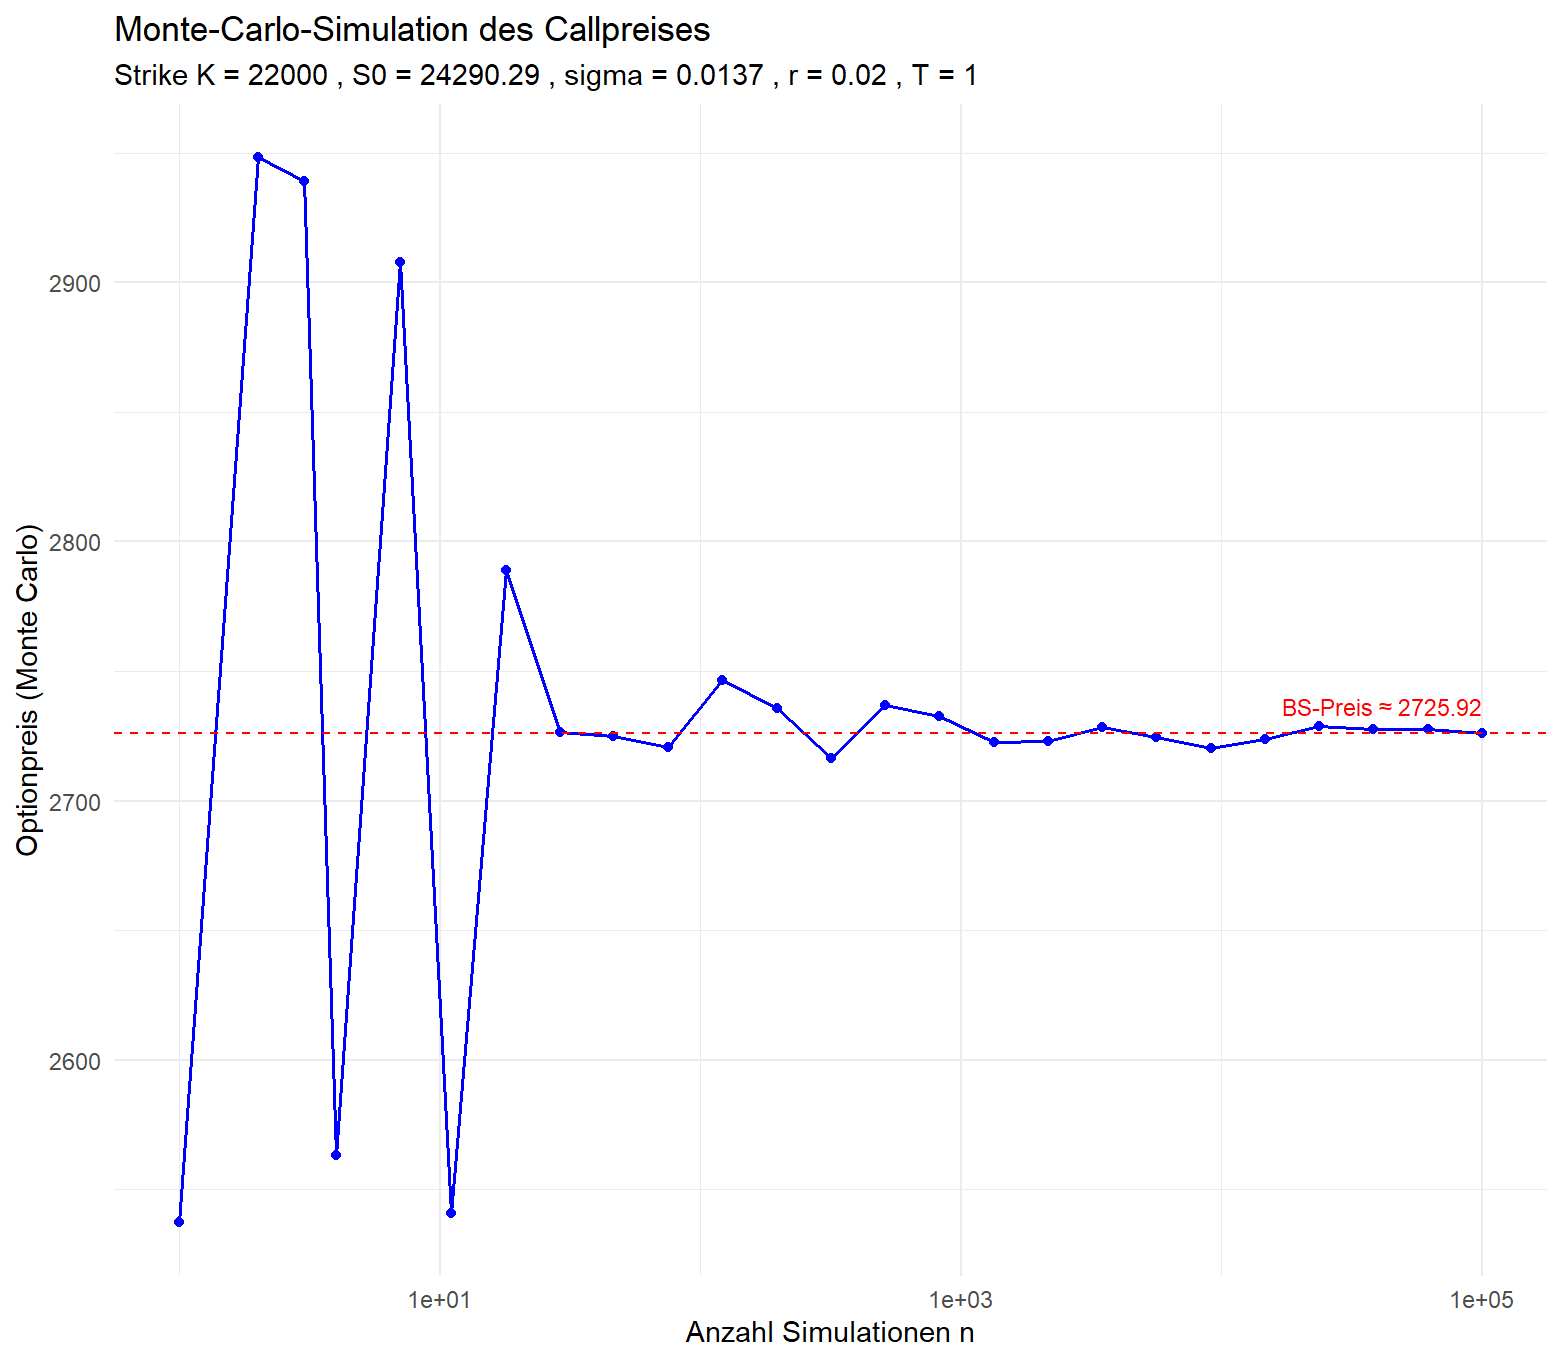
\includegraphics[width=0.9\textwidth]{images/call_dax_mc.png}
    \caption{Preis einer Call-Option auf den DAX in Abhängigkeit der Simulationsanzahl $n$ im Vergleich zur Black-Scholes-Formel}
    \label{fig:call_dax_mc}
\end{figure}

\end{bsp}

\begin{bsp}[Asiatische Optionen]
Asiatische Optionen sind Finanzderivate, bei denen die Auszahlung auf dem Durchschnittspreis
des Basiswerts über einen bestimmten Zeitraum basiert, anstatt auf dem Preis zu einem einzigen Zeitpunkt.
Die Auszahlung einer asiatischen Call-Option mit Ausübungspreis $K$ und Laufzeit $T$ ist
$$f(S_T) = \max\left(\frac{1}{T} \int_0^T S_t\,dt - K, 0\right).$$
Die Bewertung erfolgt mit dem Monte-Carlo-Verfahren, da es keine geschlossene Formel wie bei der Black-Scholes-Formel gibt.
Die Implementierung in R könnte wie folgt aussehen:

\begin{lstlisting}
Z <- matrix(rnorm(N * m), nrow=N, ncol=m) # N Pfade mit m Zeitschritten
dt <- T / m
S <- matrix(0, nrow=N, ncol=m)
S[,1] <- S0
for (j in 2:m) {
  S[,j] <- S[,j-1] * exp((r - 0.5*sigma^2)*dt + sigma*sqrt(dt)*Z[,j])
}
avg_price <- rowMeans(S) # Durchschnittspreis für jeden Pfad
payoff <- pmax(avg_price - K, 0) # Bewertungsfunktion
C <- exp(-r*T) * mean(payoff) # diskontierter Monte-Carlo-Schätzer
\end{lstlisting}

\end{bsp}